%!TEX root =  ../main.tex
\renewcommand{\columnseprule}{1.5pt}
\begin{multicols*}{2}
\rule[0.5\baselineskip]{0.4\textwidth}{1pt}
\noindent
\LabSection{Limits by Derivative}\label{sec:0804p}
\begin{exercises}{sec:0804p}
\lab{} It is not always easy to tell what a limit at infinity will be, especially with unfamiliar functions.  Consider 
$$
f(x) = \frac{4(e^x-e)}{x^{11}-1}
$$
Sketch a graph below.

\noindent
\begin{centering}
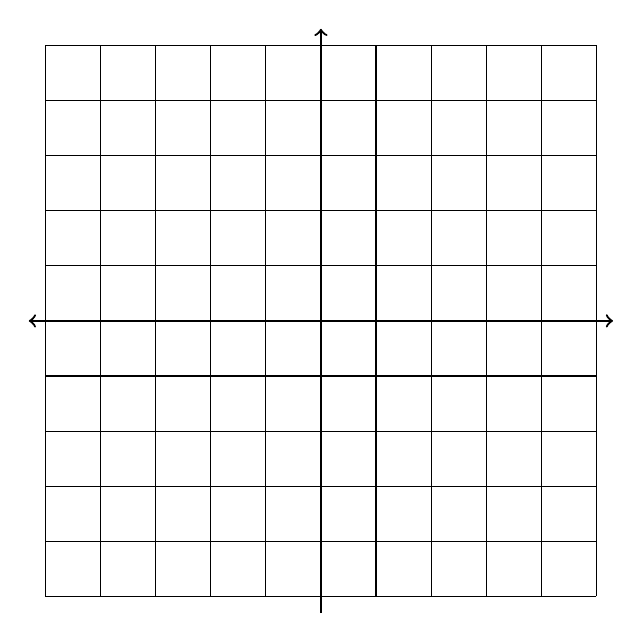
\begin{tikzpicture}[xscale=0.7,yscale=0.7]
	\draw [thick, <->] (-5.3,0) -- (5.3,0);
	\draw [thick, ->] (0,-5.3) -- (0,5.3);
	\draw [thin] (-5,-5) grid (5,5);
\end{tikzpicture}
\end{centering}

\lab{} Based off the graph, how would you answer $\lim_{x\rightarrow\infty}f(x)$?

\vspace{1cm}
\lab{} Press 2nd-WINDOW and go to TABLE SETUP.  Start at 0 and skip by 10’s.  Now press 2nd-GRAPH and look at the TABLE itself.  Describe the progression of $f(x)$ for all positive arguments.

\vspace{3cm}
\lab{} Before we tackle infinity, we should find the limit at 1.  TRACE along the graph and ZOOM-IN several time to find a numerical approximation, accurate to 3 decimal places.

\vspace{2cm}
\lab{} For every tiny step along f(x), the numerator is changing some small amount, and the denominator by a different amount.  Implicitly differentiate the numerator and the denominator separately, but write them in a fraction.

\vspace{3cm}
\lab{} Evaluate the function you made in L5 at 1.

\vspace{2cm}
\lab{} To use this method (called L’Hopital’s Rule) at infinity, repeated applications are necessary.  Differentiate the numerate and denominator separately, but write in fraction, several times until you obtain a function that is not indeterminate but infinite at infinity, confirming the TABLE.

\vspace{3cm}
\lab{} Explain in your own words what you think the point of this problem set is.

\end{exercises}
\end{multicols*}